\documentclass[11pt,a4paper]{article}
\usepackage[utf8]{inputenc}
\usepackage[T1]{fontenc}
\usepackage[polish]{babel}
\usepackage{geometry}
\usepackage{float}
\usepackage{setspace}
\usepackage{graphicx}
\newgeometry{tmargin=2cm, bmargin=2cm, lmargin=2cm, rmargin=2cm}
\author{Rafał Byczek}
\title{Mini Projekt - Mapa}
\begin{document}
\maketitle
Przesyłam Panu rozwiązanie zadania Mapa. Uwaga numer 1 - proszę używać pythona2, bo do tej wersji dostosowałem moje rozwiązanie oraz przed uruchamianiem \textbf{python2 main.py} zaleca się używanie aplikacji z konta roota, żeby w paru miejscach nie trzeba podawać hasła podczas wykonywania się lini w kodzie basha z prefiksem sudo :) Na początek mały opis co się tutaj wogóle znajduje:

\begin{itemize}
\item \textbf{./geopy} - jest to wspaniała biblioteka pythonowa pobrana z strony \\ \textbf{https://pypi.python.org/pypi/geopy}, dzięki uprzejmości tej biblioteki dostałem możliwość dostawania współrzędnych geograficznych jakichś krajów, ulic itp, które są używane w poniższych rozwiązaniach

\item \textbf{./data/data01.txt} - to jest plik udostępniony przez Pana pod nazwą \textit{data-used-autnums} zawierający informacje o numerach AS.
\item \textbf{./data/data02.txt} - to jest plik udostępniony przez Pana pod nazwą \textit{data-raw-table}, w którym są podane powiązania numerów IP z numerami AS.
\item \textbf{./data/data03.txt} - to jest plik mapujący pełne nazwy krajów na skróty dwuznakowe.
\item \textbf{./databse.py} - to jest plik, który należy uruchomić na początku. zadaniem tego programu jest odpowiednie przetworzenie plików z folderu \textit{data}, do formatu, który mi potem jest pomocny. I tak plik \textit{./data/data01.txt} ewoluuje do pliku \textbf{./data02.in}, plik \textit{./data/data02/txt} do \textbf{./data03.in} oraz plik \textit{./data/data03.txt} do \textbf{./data01.in}.
\item \textbf{./data01.in} trzyma wiersze postaci \textit{skrot\_kraju\%pelna\_nazwa\_kraju}
\item \textbf{./data02.in} trzyma wiersze postaci 
\textit{numer\_as\%skrot\_kraju\%dodatkowe\_informacje\_o\_numerze\_as}
\item \textbf{./data03.in} korzystając z informacji z pliku wiążącego ip z as trzyma wiersze następującej postaci
\textit{numer\_ip\_normalnie\%maska\_normalnie\%numer\_ip\_binarnie\%maska\_binarnie}
\end{itemize}

No i teraz mamy doczynieniaa z głównym plikiem \textbf{./main.py}. W nim się dzieje cała reszta.
Najpierw w liniach od 7-29 następuje załadowanie informacji z plików \textit{./data01.in, ./data02.in, ./data03.in} do odpowiednich słowników. Funkcja \textbf{def check(ip)} znajdująca się w liniach od 31 do 44 ma za zadanie sprawdzać czy w wczytanych danych istnieje nasz numer IP, bo te pliki nie zawierają wszystkiego. W głównej pętli programy prosimy użytkownika o podanie numeru IP. Gdy dostajemy numer IP w liniach od 63 do 91 próbujemy wycisnąć z naszych plików wszystko co można i stosowne informacje są wyświetlane na ekranie użytkownikowi. 

Druga część rozwiązania korzysta z linuxowego polecenia \textbf{whois}. W liniach od 49 do 57 jest ono używane, a za pomocą grepa do katalogu temp są wyodrębniane do plików interesujące nas informacje na temat danego numeru IP, jego numeru AS i organizacji, która zarządza tym numerem AS. Potem te dane są przetwarzane w liniach od 99 do 160 i wypisywane na ekran użytkownikowi.

Trzecia część zaś zawiera rozwiązanie korzystające z vpn i pingowania. Mamy tutaj program \textbf{./getPingTime.sh}, który uruchamiamy w postaci \textit{./getPingTime.sh miasto numer\_ip}. Za pomocą programu \textbf{./getPingTime.sh} najpierw tworzę vpn za pomocą pliku dostarczonego przez Pana nam zawierającego miasta \textit{bombay, california, frankfurt, saopaulo, sydney, tokyo, virginia}. I tak dla każdego miasta robię w tablicy routingu małe przekierowania przez podane miasto, i potem pingujemy i dla każdego miasta mierzymy średni czas przesłania pakietów. Potem każde połączenie czyści za sobą i przywraca tablice routingu do pierwotnej postaci. Zaś w pliku \textbf{./main.py} w liniach od 197 do 220 następuje przeparsowanie tego co wypisał program ping i policzenie średniego czasu na przesłanie pakietu i wypisanie użytkownikowi stosownej informacji dla każdego miasta. 

\begin{figure}
\centering
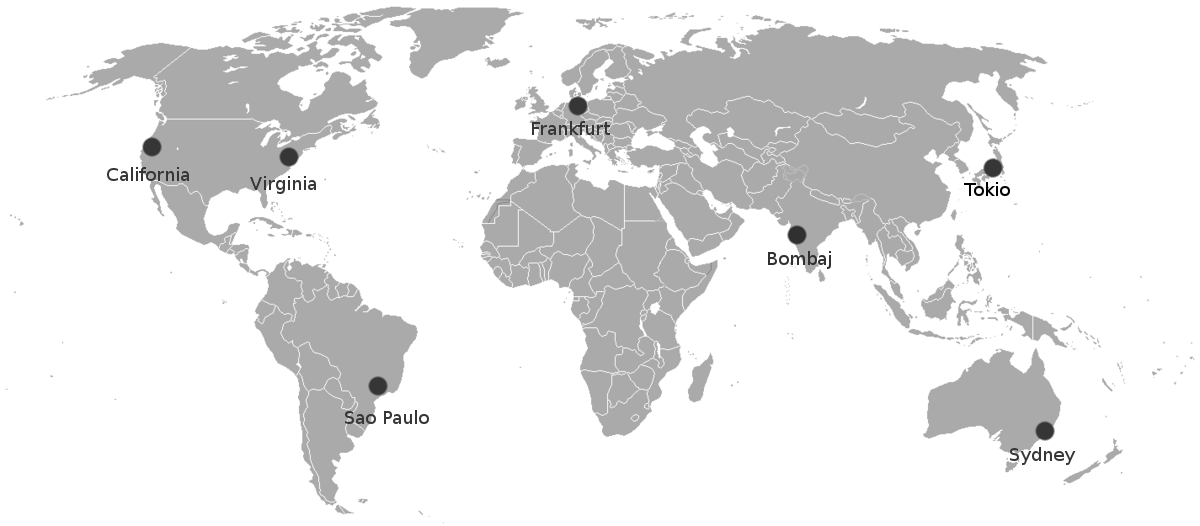
\includegraphics[scale=0.4]{mapa.png}
\end{figure}

Używając biblioteki \textbf{geopy} i znajdującego się tam pliku \textbf{./distance.py}, w którym jest między innymi zaimplementowane liczenie najkrótszej odległości na sferze zwanej \textbf{Ortodroma}. Za pomocą testów wykonanych w wykomentowanych liniach w okolicach linii 18-24, 256-259, 280-281, które brały lokalizację mojego domu i liczyły odleglości od miast \textit{bombay, california, frankfurt, saopaulo, sydney, tokyo, virginia} i czasy trwania pingów. Na podstawie tak zebranych danych uzyskałem coś na kształt
średniej prędkości \textit{internetu w powietrzu}, uzyskując około \textbf{20165129.2815 m/s}. Tej prędkości będę używał w dalszych obliczeniach. Teraz znając prędkość przepływu zapisaną w zmiennej \textbf{SREDNIA\_PREDKOSC} oraz mając czasy pingów z poszczególnych miast, jestem w stanie wyznaczyć plus minus odległość interesującego mnie numeru IP od danego miasta, co też potem ląduje w słowniku \textbf{odleglosc}, ktory to slownik trzyma teraz dla mnie pod kluczem nazwa miasta - przypuszczalna odleglosc od niego wyrażoną w metrach.

A więc mam teraz jakiś zbiór punktów na kuli ziemskiej wraz z odleglosciami od szukanego miejsca. Więc ja teraz traktuję odwrotności tych odległości jako wagi tych punktów i będę szukał środka masy dla tych punktów na kuli ziemskiej. Posłuże się w tym celu algorytmem liczenia środka masy dla punktów na kuli ziemskiej znajdującym się tutaj \textbf{http://www.geomidpoint.com/calculation.html}. Algorytm ten został zaimplementowany w pliku \textbf{main.py} w liniach od 303 do 350. Z wyliczonego środka masy za pomocą biblioteki \textbf{geopy} uzyskuję co to za miejsce na kuli ziemskiej ma takie współrzędne geograficzne jak środek masy moich punktów.

Niestety wynik ten nie jest zbyt dokładny. Dość dużym problemem jest pingowanie, bo ping np do Warszawy zajmuje tyle czasu, że równie dobrze Warszawa mogłaby być 10 razy dalej od Krakowa niż jest aktualnie. Niemniej jednak część świata, gdzie jest owy numer IP wskazuje dobrze. :)
\end{document}